
\section{Formulation for Implicit Time Steppers for ODEs and DAEs}

\label{rythmos:sec:implicit-time-steppers}

Here we consider several different classes of implicit time stepping
methods. For each class of method we show the set of general nonlinear
equations that defines a single time step and then show how a linearized
form of the equations may be formed to be solved by a Newton-type
nonlinear equation solver.

In particular, for each method, we will show how to define a set of
nonlinear equations of the form 
\begin{equation}
r(z)=0\label{rythmos:eq:r}
\end{equation}
such that when solved will define an implicit time step from $t_{k}$
to $t_{k+1}$, where $\Delta t=t_{k+1}-t_{k}$ denotes the time-step.
In addition, for each method, we will show how to use the DAE residual
evaluation $(\dot{x},x,t){}\rightarrow f$ to define the nonlinear
time step equation (\ref{rythmos:eq:r}). At the highest level, the
time step method only requires very general convergence criteria for
the time step equation (\ref{rythmos:eq:r}) and therefore great flexibility
is allowed in how the time step equation is solved. In general, the
system in (\ref{rythmos:eq:r}) must be solved such that $||x_{k+1}-x^{*}(t_{k+1})||<\eta$,
where $x_{k+1}\in\mathcal{X}$ is the computed step for the state,
$x^{*}(t_{k+1})\in\mathcal{X}$ is the exact state solution at $t_{k+1}$,
and $\eta$ is the maximum allowable local truncation error defined
by the user.

Even though the time step equation can be solved by a variety of means,
a large class of DAEs can also potentially provide support for a general
Newton-type method for solving these equations and can therefore leverage
general software for solving such problems (e.g.\ NOX). The foundation
of Newton-like methods is the ability to solve linear systems similar
to the Newton system 
\begin{equation}
\Jac{r}{z}\Delta z=-r(z_{l})
\end{equation}
where $z_{l}$ is the current candidate solution of the nonlinear
equations (which also defines the point where $\jac{r}{z}$ is evaluated)
and $\Delta z=r_{l+1}-r_{l}$ is the update direction. Line-search
Newton methods then define an update to the solution along the direction
$\Delta z$. The essential functionality needed to perform a Newton-like
method are the the abilities to evaluate the nonlinear residual $z{}\rightarrow r$
and to (approximately) solve linear systems involving the Jacobian
matrix $\jac{r}{z}$. For each type of implicit time integration method,
we will show, if possible, how to perform solves with $\jac{r}{z}$
by performing solves with the matrix 
\begin{equation}
W=\alpha\Jac{f}{\dot{x}}+\beta\Jac{f}{x},\label{rythmos:eq:W}
\end{equation}
evaluated at points $(\dot{x},x,t)$ selected by the time integration
method and where $\alpha\in\RE$ and $\beta\in\RE$ is some constants
also defined by the time integration method. Note that the matrix
$W$ above in (\ref{rythmos:eq:W_bdf}) may not necessarily exactly
represent $\jac{r}{z}$ and $z$ and $r$ may not simply lie in the
vector spaces $\mathcal{X}$ and $\mathcal{F}$ respectively; but
in many cases, they will.

The iteration matrix, $W$, is defined to be
\[
W\equiv\frac{df}{dx_{n}}=\frac{\partial\dot{x}}{\partial x_{n}}\Jac{f}{\dot{x}}+\frac{\partial x}{\partial x_{n}}\Jac{f}{x}=\alpha\Jac{f}{\dot{x}}+\beta\Jac{f}{x}
\]
where $\alpha=\partial\dot{x}/\partial x_{n}$ and $\beta=\partial x/\partial x_{n}$,
and recalling $f\left(\dot{x}(x_{n}),x(x_{n})\right)=0$.


\subsection{Backward Euler}


\subsubsection{Constant Step Size}

In Fig.~\ref{rythmos:fig:BackwardEuler-Constant-dt}, the order of
accuracy is shown for Backward Euler for the SinCos problem.

\begin{figure}[H]
\centering{}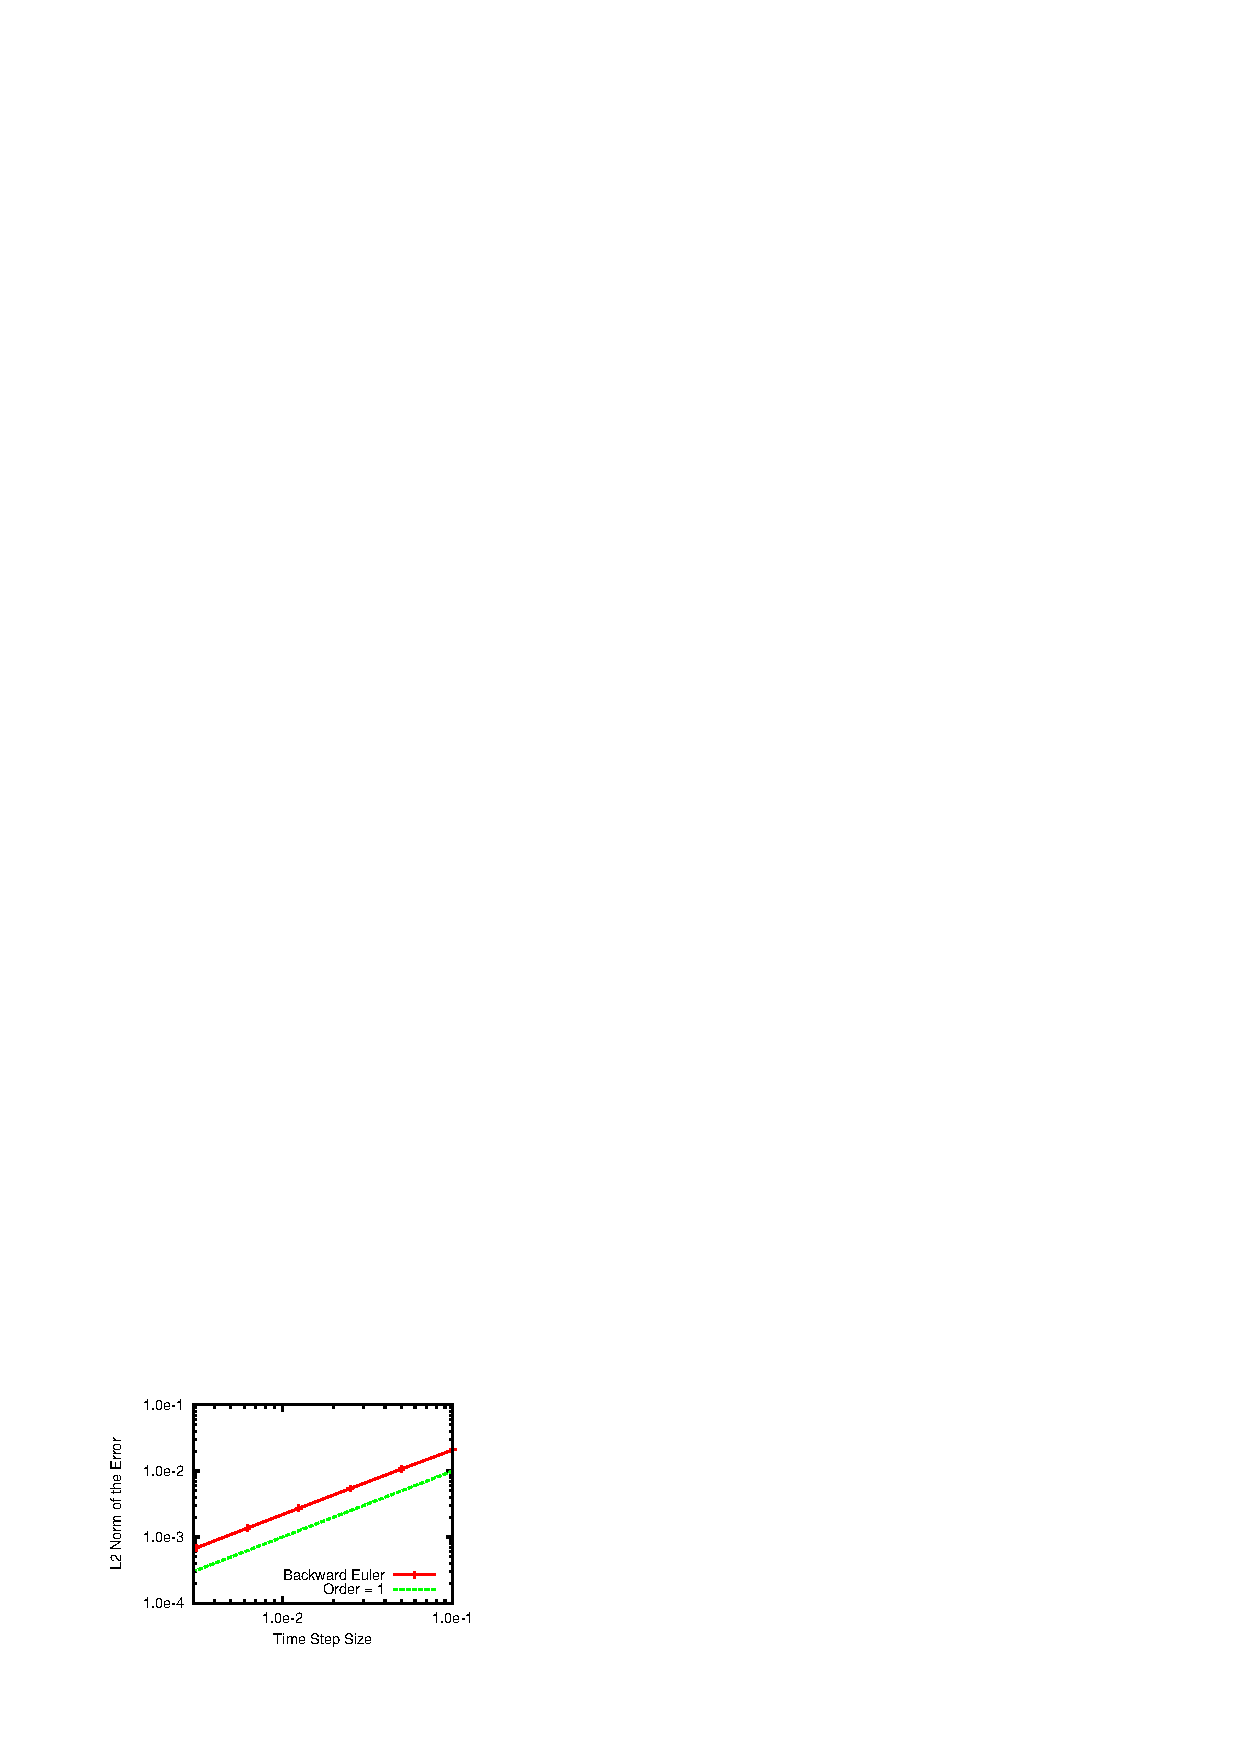
\includegraphics[scale=1.5]{figures/BackwardEuler}\caption{Order of accuracy for the SinCos Problem (Section~\ref{rythmos:sec:SinCos-Problem})
using Backward Euler.\label{rythmos:fig:BackwardEuler-Constant-dt}}
\end{figure}



\subsubsection{Variable Step Size}

A good test for variable step size is the Log-Time problem which is
defined in Sec.~\ref{rythmos:sec:Log-Time-Problem}. To adjust the
step size, the FirstOrderErrorStepControlStrategy uses the difference
between the predicted and final solution as an measure of the temporal
error and sets the next step size to maintain the user specified level
of error. Figure~\ref{rythmos:fig:BackwardEuler-Variable-dt} shows
this for the Backward Euler method for four different relative errors,
$\epsilon_{r}=$ $10^{-2}$, $10^{-3}$, $10^{-4}$, and $10^{-5}$. 

\begin{figure}[H]
\centering{}%
\begin{tabular}{cc}
a)\includegraphics[width=2.75in]{figures/BackwardEuler_FirstOrderError_var_dt_RelError=1\lyxdot 0e-2} & b)\includegraphics[width=2.75in]{figures/BackwardEuler_FirstOrderError_var_dt_RelError=1\lyxdot 0e-3}\tabularnewline
c)\includegraphics[width=2.75in]{figures/BackwardEuler_FirstOrderError_var_dt_RelError=1\lyxdot 0e-4} & d)\includegraphics[width=2.75in]{figures/BackwardEuler_FirstOrderError_var_dt_RelError=1\lyxdot 0e-5}\tabularnewline
\end{tabular}\caption{Solution and time step sizes for the Log-Time Problem (Section~\ref{rythmos:sec:Log-Time-Problem})
using Backward Euler with various relative errors in the FirstOrderErrorStepControlStrategy:
a) $\epsilon_{r}=$ a) $10^{-2}$, b) $10^{-3}$, c) $10^{-4}$, and
d) $10^{-5}$.\label{rythmos:fig:BackwardEuler-Variable-dt}}
\end{figure}


In Table~\ref{rythmos:tab:BackwardEuler-Variable-dt-Log-Time}, the
errors for this problem are shown. For each magnitude reduction in
the relative-error specification, the number of steps increases by
a factor of 2-3 and a similar reduction in the error norms and global
errors.

\begin{table}


\begin{centering}
\caption{Log-Time Errors for Backward Euler with Variable Step Size for the
Log-Time Problem.\label{rythmos:tab:BackwardEuler-Variable-dt-Log-Time}}
\begin{tabular}{|c|c|c|c|}
\hline 
$\epsilon_{r}$ & Number of Steps & Error Norm ($0\leq t_{n}\leq1$) & Global Error ($t=1$)\tabularnewline
\hline 
\hline 
$10^{-2}$ & 213 & 0.0224098 & 0.0224576\tabularnewline
\hline 
$10^{-3}$ & 563 & 0.0132322 & 0.0132634\tabularnewline
\hline 
$10^{-4}$ & 1534 & 0.00480765 & 0.00482358\tabularnewline
\hline 
$10^{-5}$ & 4168 & 0.00153523 & 0.00154173\tabularnewline
\hline 
\end{tabular}
\par\end{centering}

\end{table}


The exponential growth in the time step size, $\Delta t$, over $10^{-8}<t<1$
is approximately 8\% ($\Delta t_{n}\approx1.08\Delta t_{n-1}$), which
doubles the step size approximately every 10 time steps, and is unaffected
by the relative error, $\epsilon_{r}$. The primary effect of $\epsilon_{r}$
is to reduce $\Delta t$ over the majority of the run, except for
the initial few steps (\textasciitilde{}10). The two `blips' near
$t=10^{-9}$ are evident with all $\epsilon_{r}$, and correspond
to the locations where the curvature in the solution are large.
